\problemname{Mineraaliesiintymät}

\illustration{.3}{img/turnbull.jpg}{Kulunut mutapinta paljastaa uusia mineraaleja. Kuva: Michael D.\ Turnbull, oikeudet: CC BY-SA.}

% You handle signal processing for an extra-terrestrial mining company, and your vessel is currently approaching an asteroid. 
% Preliminary scans show the presence of $k$~mineral deposits on the asteroid, but their precise locations are unknown.

\noindent
Hoidat signaalinkäsittelyä ulkoavaruuden kaivosyhtiössä, ja avaruusaluksesi lähestyy parhaillaan asteroidia.
Alustavat skannaukset näyttävät, että asteroidilla on $k$~mineraaliesiintymää, mutta niiden tarkat sijainnit ei ole tiedossa.

\medskip

% The surface of the asteroid can be seen as a grid of integer coordinates.
% Each of the mineral deposits is located at unknown integer coordinates such that the $i$th deposit has coordinates $(x_i, y_i)$ with  
% $-b \le x_i \le b$ and $-b\le y_i \le b$ %constraint:depositcoords
% for some integer $b$ corresponding to the size of your initial scan.

Asteroidin pinta voidaan nähdä kokonaislukukoordinaattisena ruudukkona, jossa
$i$:s mineraaliesiintymä sijaitsee tuntemattomissa koordinaateissa $(x_i, y_i)$, joille pätee 
$-b \le x_i \le b$ and $-b\le y_i \le b$ %constraint:depositcoords
jollakin kokonaisluvulla $b$, joka vastaa alustavan skannauksen kokoa.

% To determine the precise locations of the mineral deposits, you may send probes to the surface of the asteroid. 
% The probes are sent out in waves of several probes at once.

Selvittääksesi mineraaliesiintymien tarkat sijainnit, voit lähettää luotaimia asteroidin pinnalle.
Luotaimet lähetetään useiden luotainten aalloissa.

% Say you sent a wave of $d$~probes to the surface at coordinates $(s_j,t_j)$ for $1\leq j\leq d$.
% When a probe arrives at its coordinates, it determines the Manhattan distances to each of the $k$~mineral deposits and sends the distances back to the ship. 
% All data packets arrive at the same time, and it is not possible to determine which probes returned which distances. 
% Thus the wave returns the $k\cdot d$ integer distances
% \[|x_i-s_j| + |y_i - t_j| \qquad\text{for all } i \in \{1,\ldots,k\} \text{ and } j \in\{ 1,\ldots,d\}\,.\]

Sanotaan, että lähetät pinnalle $d$:n~luotaimen aallon koordinaatteihin $(s_j, t_j)$, kun $1\leq j\leq d$.
Kun luotain saapuu koordinaatteihinsa, se mittaa Manhattan-etäisyyden jokaiseen $k$:sta~mineraaliesiintymästä ja lähettää etäisyydet takaisin alukselle.
Kaikki etäisyystiedot saapuvat samaan aikaan, eikä ole mahdollista selvittää, mikä luotain palautti mitkäkin etäisyydet.
Luotainaalto palauttaa siis $k \cdot d$ kokonaislukuetäisyyttä
\[|x_i-s_j| + |y_i - t_j|, \qquad\text{missä } i \in \{1,\ldots,k\} \text{ ja } j \in\{ 1,\ldots,d\}\,.\]

% You need to minimise the number of waves of probes that is sent to the surface.
Tehtäväsi on minimoida pinnalle lähetettävien luotainaaltojen määrä.

\section*{Interaktio}

Tämä on interaktiivinen tehtävä.
Interaktio alkaa sillä, että luet yhden rivin, joka sisältää kolme kokonaislukua $b$, $k$ ja $w$:
ruudukon raja~$b$,
mineraaliesiintymien määrä~$k$
ja suurin mahdollinen määrä luotainaaltoja $w$.

Tämän jälkeen voit tehdä yhteensä $w$ kyselyä, joista jokainen vastaa yhden luotainaallon lähettämistä.
% A query consists of \texttt{?} followed by $2d$ integers separated by space,
% such as ``\texttt{?} $s_1$ $t_1$ $\cdots$ $s_d$ $t_d$'',
% where the number~$d$ of probes in this wave must satisfy
Kysely koostuu merkistä \texttt{?}, jota seuraa $2d$ välilyönneillä erotettua kokonaislukua,
esimerkiksi ``\texttt{?} $s_1$ $t_1$ $\cdots$ $s_d$ $t_d$'',
jossa luotainten määrälle $d$ täytyy päteä
$1\leq d\leq 2000$. % constraint:wavesize
% The values $(s_i,t_i)$ are interpreted as the coordinates of the $i$th probe and must satisfy
% $-10^8 \leq s_i \leq 10^8$ and $-10^8 \leq t_i \leq 10^8$. % constraint:probecoordinates
% The response is a single line with $k \cdot d$ integers in non-decreasing order: all pairs of Manhattan distances between the mineral deposits and the probe coordinates.
Arvot $(s_i,t_i)$ tulkitaan $i$:nnen luotaimen koordinaatteina ja niille täytyy päteä
$-10^8 \leq s_i \leq 10^8$ ja $-10^8 \leq t_i \leq 10^8$. % constraint:probecoordinates
Vastaus on yksi rivi, joka sisältää $k \cdot d$ kokonaislukua
ei-vähenevässä järjestyksessä: % FIXME: Onko tämä hyvä käännös? UPD: Nyt ainakin selkeämpi?
kaikki parit Manhattan-etäisyyksiä mineraaliesiintymien ja luotainten välillä.
% The total number of probes across all waves may not exceed
% $2\cdot 10^4.$ % constraint:totalprobes
Kaikissa aalloissa lähetettyjen luotainten kokonaismäärä ei saa ylittää
$2\cdot 10^4.$ % constraint:totalprobes

% Interaction ends with you printing a single line consisting of \texttt{!} followed by $k$ points $x_1, y_1, x_2, y_2, \ldots x_k, y_k$, separated by space.
Interaktio loppuu riviin, joka koostuu merkistä \texttt{!} ja $k$:sta pisteestä $x_1, y_1, x_2, y_2, \ldots x_k, y_k$, välilyönneillä erotettuina.
% This must be your last line of output.
Tämän tulee olla tulosteen viimeinen rivi.

% Your submission is considered correct if you print all locations of the mineral deposits.
Ratkaisusi katsotaan oikeaksi, jos se tulostaa jokaisen mineraaliesiintymän sijainnin oikein.
Voit tulostaa ne missä tahansa järjestyksessä.

\section*{Rajoitukset ja pisteytys}

Kaikille testitapauksille pätee
$1\leq b \leq 10^8$, % constraint:b
$1 \leq k \leq 20$, % constraint:k
ja
$2 \le w \le 10^4$. % constraint:w

Ratkaisu testataan testiryhmillä, joista kullakin on oma pistemäärä.
Jokainen testiryhmä sisältää joukon testitapauksia.
Ryhmän pisteet saa vain, jos ratkaisee kaikki sen testitapaukset.
Tehtävän lopullinen pistemäärä on suurin yksittäisen lähetyksen pistemäärä.

\medskip
\begin{tabular}{lll}
Ryhmä & Pisteet & Rajoitukset \\\hline
  $1$ & $9$ & $k = 1, w = 10^4$\\
  $2$ & $19$ & $w \ge 500$\\
  $3$ & $11$ & $w \ge 210$\\
  $4$ & $7$ & $w \ge 130$\\
  $5$ & $20$ & $w \ge 3$, $b \le 10^4$\\
  $6$ & $15$ & $w \ge 3$, $b \le 10^7$\\
  $7$ & $19$ & \emph{Ei muita rajoituksia}
\end{tabular}

\section*{Esimerkki}

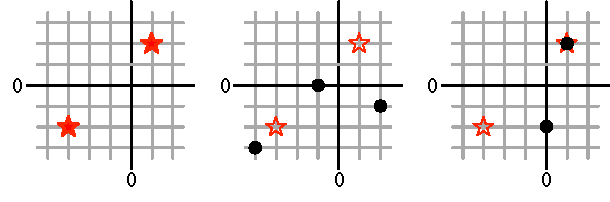
\includegraphics[width=.6\textwidth]{img/sample1.pdf}

% In this example, there are $k=2$ mineral deposits at positions $(1,2)$ and $(-3,-2)$, shown as red stars.
Tässä esimerkissä on $k=2$ mineraaliesiintymää, jotka sijaitsevat pisteissä $(1,2)$ ja $(-3,-2)$, merkitty punaisilla tähdillä.
Ensimmäisessä aallossa voisit lähettää $d=3$ luotainta pisteisiin $(-4,-3)$, $(-1, 0)$ ja $(2,-1)$, merkitty mustilla pisteillä.
Tällöin aalto palauttaisi $6$ etäisyyttä \[
  2, 4, 4, 4, 6, 10\,.
\]
Seuraavalla aallolla voisit lähettää $d=2$ luotainta pisteisiin $(1,2)$ ja $(0,-2)$.
Tällöin aalto palauttaisi $4$ etäisyyttä \[
  0, 3, 5, 8\,.
\]
